\documentclass{amsart}
\setlength{\textheight}{9in}
\setlength{\topmargin}{-0.25in}
\setlength{\textwidth}{7in}
\setlength{\evensidemargin}{-0.25in}
\setlength{\oddsidemargin}{-0.25in}
\usepackage{aaai}
\usepackage{amsfonts}
\usepackage[utf8]{inputenc}
\usepackage[T1]{fontenc}
\usepackage{graphicx} 
\usepackage[export]{adjustbox}
% needed to include these graphics
%\graphicspath{{./Pictures/}}      % only in case you want to keep the pictures in a separate
                                  % subdirectory; also see the appropriate line below
\usepackage{caption}
\usepackage{subcaption}
\usepackage{float}
\usepackage{framed}
\newcounter{temp}
\theoremstyle{definition}
\newtheorem{Thm}{Theorem}
\newtheorem{Prob}{Problem}
\newtheorem*{Def}{Definition}
\newtheorem*{Ans}{Answer}
\newcommand{\dis}{\displaystyle}
\newcommand{\dlim}{\dis\lim}
\newcommand{\dsum}{\dis\sum}
\newcommand{\dint}{\dis\int}
\newcommand{\ddint}{\dint\!\!\dint}
\newcommand{\dddint}{\dint\!\!\dint\!\!\dint}
\newcommand{\dt}{\text{d}t}
\newcommand{\dA}{\text{d}A}
\newcommand{\dV}{\text{d}V}
\newcommand{\dx}{\text{d}x}
\newcommand{\dy}{\text{d}y}
\newcommand{\dz}{\text{d}z}
\newcommand{\dw}{\text{d}w}
\newcommand{\du}{\text{d}u}
\newcommand{\dv}{\text{d}v}
\newcommand{\ds}{\text{d}s}
\newcommand{\dr}{\text{d}r}
\newcommand{\dth}{\text{d}\theta}
\newcommand{\bbR}{\mathbb{R}}
\newcommand{\bbN}{\mathbb{N}}
\newcommand{\bbQ}{\mathbb{Q}}
\newcommand{\bbZ}{\mathbb{Z}}
\newcommand{\bbC}{\mathbb{C}}
\newcommand{\dd}[2]{\dfrac{\text{d}#1}{\text{d}#2}}
\newcommand{\dydx}{\dfrac{\text{d}y}{\text{d}x}}
\renewcommand{\labelenumi}{{\normalfont \arabic{enumi}.}}
\renewcommand{\labelenumii}{{\normalfont \alph{enumii}.}}
\renewcommand{\labelenumiii}{{\normalfont \roman{enumiii}.}}
\font \bggbf cmbx18 scaled \magstep2
\font \bgbf cmbx10 scaled \magstep2
\usepackage{fancyhdr}
\usepackage{lipsum}
\usepackage{amsmath}
\usepackage{empheq}
\newcommand*\widefbox[1]{\fbox{\hspace{2em}#1\hspace{2em}}}
% Clear the header and footer
\fancyhead{}
\fancyfoot{}
% Set the right side of the footer to be the page number
\rfoot{\thepage}
\fancyhf{}
\pagestyle{fancy}
\begin{document}



%%%%%%%%%%%%%%%%%%%%%%%%%%%%%%%%%%%%%%%%%%%%%%%%%%%%%%%%%%%%%%%%%%%%%%%%%%%%%%%%%%%%%%%%%%%%%%%%%%%%%%%%%%%%%%%%%%%%%%%%%%%
%                                                                                                         Title Information
%%%%%%%%%%%%%%%%%%%%%%%%%%%%%%%%%%%%%%%%%%%%%%%%%%%%%%%%%%%%%%%%%%%%%%%%%%%%%%%%%%%%%%%%%%%%%%%%%%%%%%%%%%%%%%%%%%%%%%%%%%%
\LARGE{CIS 730: Artificial Intelligence}
 
\large
Project Report
 
John Boyington
\newline
\bigskip

%%%%%%%%%%%%%%%%%%%%%%%%%%%%%%%%%%%%%%%%%%%%%%%%%%%%%%%%%%%%%%%%%%%%%%%%%%%%%%%%%%%%%%%%%%%%%%%%%%%%%%%%%%%%%%%%%%%%%%%%%%%







%%%%%%%%%%%%%%%%%%%%%%%%%%%%%%%%%%%%%%%%%%%%%%%%%%%%%%%%%%%%%%%%%%%%%%%%%%%%%%%%%%%%%%%%%%%%%%%%%%%%%%%%%%%%%%%%%%%%%%%%%%%
%                                                                                            Objectives & Problem Statement
%%%%%%%%%%%%%%%%%%%%%%%%%%%%%%%%%%%%%%%%%%%%%%%%%%%%%%%%%%%%%%%%%%%%%%%%%%%%%%%%%%%%%%%%%%%%%%%%%%%%%%%%%%%%%%%%%%%%%%%%%%%

\section{Objectives \& Problem Statement}

%%%%%%%%%%%%%%%%%%%%%%%%%%%%%%%%%%%%%%%%%%%%%%%%%%%%%%%%%%%%%%%%%%%%%%%%%%%%%%%%%%%%%%%%%%%%%%%%%%%%%%%%%%%%%%%%%%%%%%%%%%%

StarCraft II is a popular competetive real-time strategy game.
To play successfully, players have to manage the game on both the micro-level with combat and structure placement and also at the macro-level making long-term strategic descisions.
The game is partially-observable, so exploration is required, several actions are available to the player at any given moment, things like movement and attacking happen in a continuous space and there are countless strategies used successfully.
For artificial intelligence, this game provides an excellent opportunity for research.
Recently, this game has been presented as a grand challenge in AI by DeepMind and Blizzard.

For the class project, the topic chosen was to develop a game-playing agent to master some component of this game.
More specificly, the plan was to develop a neural network to mimic the behavior of some scripted bot in the minigame `DefeatRoaches' in StarCraft II.
The hope is that through this research, more information might be gained on the process of learning through observing the action of others.
Large ammounts of replay data is available currently, including much from high-level players.
This data, in conjunction with these learned techniques may hold the key to teaching a machine to master the game.

Before starting the task there were a number of competencies I needed to develop before being able to actually the bot.
First, I would need to learn to use the StarCraft api that Blizzard and DeepMind had produced.
This python-based interface gives access to large ammounts of in-game information, like state variables and available actions, all provided in easy-to-use {\tt numpy} arrays.
This format is designed specifically with AI development in mind, and presents observation data and actions in ways that mimick human-like interpretation.

Learning Tensorflow was also necessary for the creation of the agent's neural network.
It's implementation allowed for the relatively simple creation and training of neural networks using keras.
Included in the appendix of this report is an example demonstrating the functionality of keras.

%%%%%%%%%%%%%%%%%%%%%%%%%%%%%%%%%%%%%%%%%%%%%%%%%%%%%%%%%%%%%%%%%%%%%%%%%%%%%%%%%%%%%%%%%%%%%%%%%%%%%%%%%%%%%%%%%%%%%%%%%%%






%%%%%%%%%%%%%%%%%%%%%%%%%%%%%%%%%%%%%%%%%%%%%%%%%%%%%%%%%%%%%%%%%%%%%%%%%%%%%%%%%%%%%%%%%%%%%%%%%%%%%%%%%%%%%%%%%%%%%%%%%%%
%                                                                                                 Background & Related Work
%%%%%%%%%%%%%%%%%%%%%%%%%%%%%%%%%%%%%%%%%%%%%%%%%%%%%%%%%%%%%%%%%%%%%%%%%%%%%%%%%%%%%%%%%%%%%%%%%%%%%%%%%%%%%%%%%%%%%%%%%%%

\section{Background \& Related Work}

%%%%%%%%%%%%%%%%%%%%%%%%%%%%%%%%%%%%%%%%%%%%%%%%%%%%%%%%%%%%%%%%%%%%%%%%%%%%%%%%%%%%%%%%%%%%%%%%%%%%%%%%%%%%%%%%%%%%%%%%%%%

It was in August 2017 that the paper introducing SC2LE (StarCraft II Learning Environment) was published and since then several papers have been published detailing methods used to approach the game.
Within the paper itself was several baseline results published from the application of standard reinforcement learning (RL) algorithms.
Micro behaviors were considered by Liu et. al. who used a influence maps and potential fields to teach an agent various combat techniques. (cite)
Makar et. al. studied hierarchical multi-agent RL which broke down and decentralized learning tasks handled by separate agents.

Outside of AI, StarCraft II bot development has been happening for a long time now.
A paper by Onta\~n\`on et. al. compares the performance and architecture of the most competetive of these bots.


%%%%%%%%%%%%%%%%%%%%%%%%%%%%%%%%%%%%%%%%%%%%%%%%%%%%%%%%%%%%%%%%%%%%%%%%%%%%%%%%%%%%%%%%%%%%%%%%%%%%%%%%%%%%%%%%%%%%%%%%%%%









%%%%%%%%%%%%%%%%%%%%%%%%%%%%%%%%%%%%%%%%%%%%%%%%%%%%%%%%%%%%%%%%%%%%%%%%%%%%%%%%%%%%%%%%%%%%%%%%%%%%%%%%%%%%%%%%%%%%%%%%%%%
%                                                                                                               Methodology
%%%%%%%%%%%%%%%%%%%%%%%%%%%%%%%%%%%%%%%%%%%%%%%%%%%%%%%%%%%%%%%%%%%%%%%%%%%%%%%%%%%%%%%%%%%%%%%%%%%%%%%%%%%%%%%%%%%%%%%%%%%

\section{Methodology}

%%%%%%%%%%%%%%%%%%%%%%%%%%%%%%%%%%%%%%%%%%%%%%%%%%%%%%%%%%%%%%%%%%%%%%%%%%%%%%%%%%%%%%%%%%%%%%%%%%%%%%%%%%%%%%%%%%%%%%%%%%%

The structure of the code will be considered within this section, as well as any techniques applied at various levels of implementation.
The highest level script it {\tt defeat\_roaches.py}.
It can be invoked with a command line arg, either {\tt learn} or {\tt log}.
This will select the whether you want the scripted bot, or the neural network to play the game.
Each agent is subclassed from a pysc2agent class type and then the action used at each timestep is produced using the {\tt step} method.
At the highest level, you can choose things like the ammount of ingame steps before an action execution, where mine is set to 1.
It's at this level, too that a {\tt Data\_Container} object is created and passed to agents.
This handles the access, logging, and handling of data produced by scripty and used by neural boi.

For this particular problem, the observation data used was twofold.
Because of the nature of the training bot, I needed access to two different value maps.
The first, was the unit id to distinguish who owned which units.
The second was the unit health so I could target the unit with lowest health.
This data went through a series of transformations.
First, all values were scaled to between 0 and 1.
Because for attacking we didn't need position of friendly units, so all values associated with friendlies were reduced to 0.
Due to size restraints then, the data was compressed from 124x124 to 31x31.

The action space was formulated as a series of classes.
Due to the continuous space we were in, the action space was discretized so there were 30x25 attack locations.
These (x, y) pairs were flattened and then enumerated.
Each ``action id'' became a separate class the the network would attempt to train.

The {\tt data.py} file in the repo contains the {\tt Data\_Container} object.
This object accepts a {\tt timestep} as given by the api and then grabs the obs info needed.
It also accepts as an arguement an {\tt action\_id} which logs the action taken by the scripted bot.
This data is then stored in a numpy array and saved to a file after a single game is finished.

The scripted bot was designed with two things in mind.
The first is simplicity, as it will be easier to see if the learning bot is properly mimicking its actions.
The second, is that it was designed in a way to exhibit a series of micro behaviors.
The algorithm targets the enemy with lowest health.
Ties are broken with y position.
This will focus down enemies that are the weakest to quickly remove their damage source.
The tiebreaker encourages the bot to flank the enemy units, a behavior that would be present in the learner if learned right.

After logging the data, it is given to the learning bot.
This bot will process the data and try to memorize the actions associated with each observation with its neural network.
Because the network will output a class {\tt action\_id}, it simply needs retransformed into 2D (x, y) values and then the agent will attack there.
The network has no hidden layers, just a length 1922 input and the 750 output nodes with relu activation.

For the experiment, there was a total of 51433 of traning data arrays.
The data was shuffled before being given to the network and then trained with a batch size of 64 and 3 epochs.
Both the training bot and learning bot were allowed to play 5 games each and the scores of each were recorded.


%%%%%%%%%%%%%%%%%%%%%%%%%%%%%%%%%%%%%%%%%%%%%%%%%%%%%%%%%%%%%%%%%%%%%%%%%%%%%%%%%%%%%%%%%%%%%%%%%%%%%%%%%%%%%%%%%%%%%%%%%%%








%%%%%%%%%%%%%%%%%%%%%%%%%%%%%%%%%%%%%%%%%%%%%%%%%%%%%%%%%%%%%%%%%%%%%%%%%%%%%%%%%%%%%%%%%%%%%%%%%%%%%%%%%%%%%%%%%%%%%%%%%%%
%                                                                                                                   Results
%%%%%%%%%%%%%%%%%%%%%%%%%%%%%%%%%%%%%%%%%%%%%%%%%%%%%%%%%%%%%%%%%%%%%%%%%%%%%%%%%%%%%%%%%%%%%%%%%%%%%%%%%%%%%%%%%%%%%%%%%%%

\section{Results}

%%%%%%%%%%%%%%%%%%%%%%%%%%%%%%%%%%%%%%%%%%%%%%%%%%%%%%%%%%%%%%%%%%%%%%%%%%%%%%%%%%%%%%%%%%%%%%%%%%%%%%%%%%%%%%%%%%%%%%%%%%%

% results table
\begin{table}[]
\caption{Comparison of the scores earned by both the scripted bot and the neural network in five games.}
\label{tab:scores}
\begin{tabular}{|l|l|l|}
\hline
Game & Scripted Bot & ANN  \\ \hline
1    & 126          & -8   \\ \hline
2    & 57           & 0    \\ \hline
3    & 117          & 2    \\ \hline
4    & 292          & 0    \\ \hline
5    & 210          & -8   \\ \hline
Avg. & 160.4        & -2.8 \\ \hline
\end{tabular}
\end{table}


Table \ref{tab:scores} shows the results from both of the bots.
The scripted bot demonstrated good performance, receiving an average score of [AVERAGE SCORE] and a maximum score of 292.
For the learning bot, however, it had an average score of [AVERAGE SCORE] and only a maximum score of 2.
The average accuracy for the learning bot was [AVG ACCURACY].
Qualitatively, when the accuracy was on the order of 1e-3, the agent would more confidently select an inaccurate point on the screen, cluster around that point and eliminate friendly units.
When the accuracy was closer to 1e-5, the agents actions seemed entirely stochastic.


%%%%%%%%%%%%%%%%%%%%%%%%%%%%%%%%%%%%%%%%%%%%%%%%%%%%%%%%%%%%%%%%%%%%%%%%%%%%%%%%%%%%%%%%%%%%%%%%%%%%%%%%%%%%%%%%%%%%%%%%%%%






%%%%%%%%%%%%%%%%%%%%%%%%%%%%%%%%%%%%%%%%%%%%%%%%%%%%%%%%%%%%%%%%%%%%%%%%%%%%%%%%%%%%%%%%%%%%%%%%%%%%%%%%%%%%%%%%%%%%%%%%%%%
%                                                                                                                   Summary
%%%%%%%%%%%%%%%%%%%%%%%%%%%%%%%%%%%%%%%%%%%%%%%%%%%%%%%%%%%%%%%%%%%%%%%%%%%%%%%%%%%%%%%%%%%%%%%%%%%%%%%%%%%%%%%%%%%%%%%%%%%

\section{Summary}

%%%%%%%%%%%%%%%%%%%%%%%%%%%%%%%%%%%%%%%%%%%%%%%%%%%%%%%%%%%%%%%%%%%%%%%%%%%%%%%%%%%%%%%%%%%%%%%%%%%%%%%%%%%%%%%%%%%%%%%%%%%

Clearly, the learning agent was not successful.
There were a number of hinderences that caused this.
First, to classify that number of classes, the dataset was too small.
Not only, that, but there was a large number of actions that were never taken by the scripted agent and therefore no data at all to train those.
Also, the action space enumeration orthogonalized the actions, meaning that it sacrificed its 2d nature.
Even though two attack target squares may be right next to eachother, they need separate data to train.
Ideally, there would be some correlation between nearby attack targets that would allow for easier training.

In future work, using attack policies may be better.
This would drastically reduce the number of classes needed to train.
It would change the nature  of the problem, but ultimately be more useful.
Also reinforcement techniques may be better suited for this problem.

Ultimately, the problem still remains unsolved but strides were made.
The challenges provided by large datasizes seemed to be properly addressed by the image compression.
Future work will happen.

%%%%%%%%%%%%%%%%%%%%%%%%%%%%%%%%%%%%%%%%%%%%%%%%%%%%%%%%%%%%%%%%%%%%%%%%%%%%%%%%%%%%%%%%%%%%%%%%%%%%%%%%%%%%%%%%%%%%%%%%%%%







%%%%%%%%%%%%%%%%%%%%%%%%%%%%%%%%%%%%%%%%%%%%%%%%%%%%%%%%%%%%%%%%%%%%%%%%%%%%%%%%%%%%%%%%%%%%%%%%%%%%%%%%%%%%%%%%%%%%%%%%%%%
%                                                                                                                References
%%%%%%%%%%%%%%%%%%%%%%%%%%%%%%%%%%%%%%%%%%%%%%%%%%%%%%%%%%%%%%%%%%%%%%%%%%%%%%%%%%%%%%%%%%%%%%%%%%%%%%%%%%%%%%%%%%%%%%%%%%%

\section{References}

%%%%%%%%%%%%%%%%%%%%%%%%%%%%%%%%%%%%%%%%%%%%%%%%%%%%%%%%%%%%%%%%%%%%%%%%%%%%%%%%%%%%%%%%%%%%%%%%%%%%%%%%%%%%%%%%%%%%%%%%%%%






%%%%%%%%%%%%%%%%%%%%%%%%%%%%%%%%%%%%%%%%%%%%%%%%%%%%%%%%%%%%%%%%%%%%%%%%%%%%%%%%%%%%%%%%%%%%%%%%%%%%%%%%%%%%%%%%%%%%%%%%%%%
%                                                                                                                  Appendix
%%%%%%%%%%%%%%%%%%%%%%%%%%%%%%%%%%%%%%%%%%%%%%%%%%%%%%%%%%%%%%%%%%%%%%%%%%%%%%%%%%%%%%%%%%%%%%%%%%%%%%%%%%%%%%%%%%%%%%%%%%%

\section{Appendix}

%%%%%%%%%%%%%%%%%%%%%%%%%%%%%%%%%%%%%%%%%%%%%%%%%%%%%%%%%%%%%%%%%%%%%%%%%%%%%%%%%%%%%%%%%%%%%%%%%%%%%%%%%%%%%%%%%%%%%%%%%%%

Here's an example of me learning tensorflow.
It can be found in the repository.
I followed the training on the tensorflow website.
Those instructions will go here.


\begin{figure}[h!]
    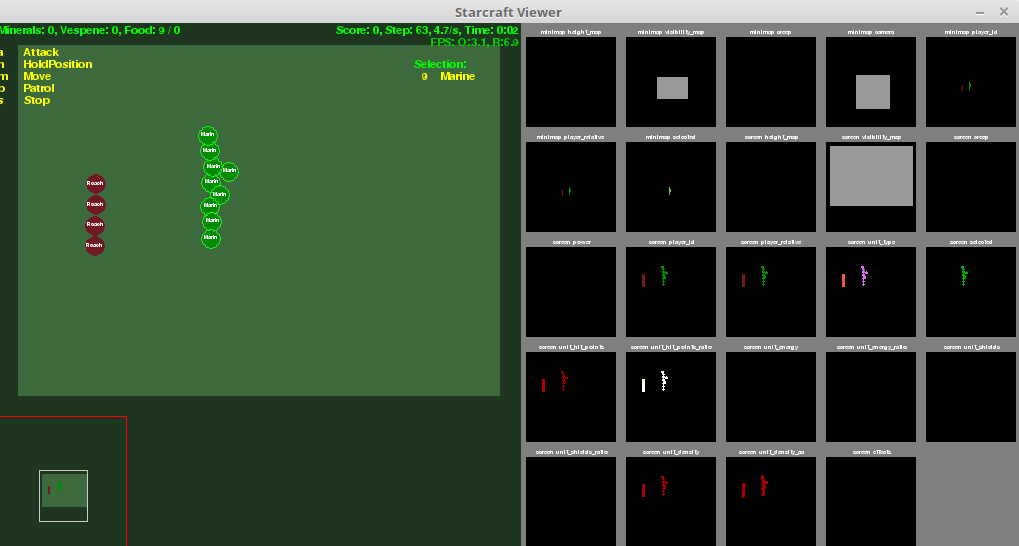
\includegraphics[width=1.0\linewidth]{gameplay}
    \caption{The pysc2 api visualized, showing the gameplay on the left and all of the feature screens on the right. Marines are represented by the green circles and the roaches by the red circles.}
\end{figure}


\begin{figure}[h!]
    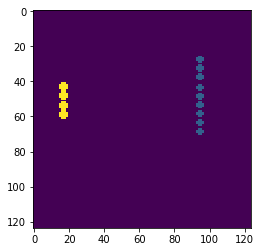
\includegraphics[width=1.0\linewidth]{fine}
    \caption{An image representing the {\tt player\_id} feature screen.}
\end{figure}

\begin{figure}[h!]
    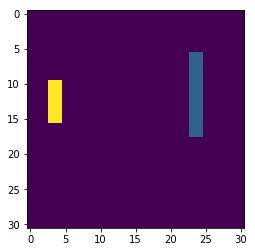
\includegraphics[width=1.0\linewidth]{course}
    \caption{An image representing the {\tt player\_id} feature screen, after have underwent the image compression techniques described above.}
\end{figure}

%%%%%%%%%%%%%%%%%%%%%%%%%%%%%%%%%%%%%%%%%%%%%%%%%%%%%%%%%%%%%%%%%%%%%%%%%%%%%%%%%%%%%%%%%%%%%%%%%%%%%%%%%%%%%%%%%%%%%%%%%%%










\end{document}
